% Created 2024-02-09 Fri 16:20
% Intended LaTeX compiler: pdflatex
\documentclass[11pt]{article}
\usepackage[utf8]{inputenc}
\usepackage[T1]{fontenc}
\usepackage{graphicx}
\usepackage{grffile}
\usepackage{longtable}
\usepackage{wrapfig}
\usepackage{rotating}
\usepackage[normalem]{ulem}
\usepackage{amsmath}
\usepackage{textcomp}
\usepackage{amssymb}
\usepackage{capt-of}
\usepackage{hyperref}
\usepackage{minted}
\usepackage[a4paper,margin=20mm]{geometry}
\usepackage{amsmath}
\usepackage{amsfonts}
\usepackage{bm}
\usepackage{minted}
\usemintedstyle{emacs}
\usepackage[T1]{fontenc}
\usepackage[scaled]{beraserif}
\usepackage[scaled]{berasans}
\usepackage[scaled]{beramono}
\newcommand{\tr}{\textsf{T}}
\newcommand{\grad}{\bm{\nabla}}
\newcommand{\av}[2][]{\mathbb{E}_{#1\!}\left[ #2 \right]}
\newcommand{\Prob}[2][]{\mathbb{P}_{#1\!}\left[ #2 \right]}
\newcommand{\logg}[1]{\log\!\left( #1 \right)}
\newcommand{\e}[1]{{\rm e}^{#1}}
\newcommand{\dd}{\mathrm{d}}
\DeclareMathAlphabet{\mat}{OT1}{cmss}{bx}{n}
\newcommand{\normal}[2]{\mathcal{N}\!\left(#1 \big| #2 \right)}
\newcounter{eqCounter}
\setcounter{eqCounter}{0}
\newcommand{\explanation}{\setcounter{eqCounter}{0}\renewcommand{\labelenumi}{(\arabic{enumi})}}
\newcommand{\eq}[1][=]{\stepcounter{eqCounter}\stackrel{\text{\tiny(\arabic{eqCounter})}}{#1}}
\newcommand{\argmax}{\mathop{\mathrm{argmax}}}
\author{Adam Prügel-Bennett}
\date{\today}
\title{Advanced Machine Learning Subsidary Notes\\\medskip
\large Lecture 23: Probabilistic Inference}
\hypersetup{
 pdfauthor={Adam Prügel-Bennett},
 pdftitle={Advanced Machine Learning Subsidary Notes},
 pdfkeywords={},
 pdfsubject={},
 pdfcreator={Emacs 27.1 (Org mode 9.3)}, 
 pdflang={English}}
\begin{document}

\maketitle


\section{Keywords}
\label{sec:org42594cf}
\begin{itemize}
\item Hierarchical Models, Mixture of Gaussians, Expectation Maximisation
\end{itemize}


\section{Main Points}
\label{sec:org7d3b6af}

\subsection{Laws of Probability}
\label{sec:org15b8190}
\begin{itemize}
\item We  quickly review probabilities (you should know all this)
\item Probabilities and events
\begin{itemize}
\item We typically associate probabilities with events
\item The probability of an event lie between 0 and 1
\item If the set of events \(\mathcal{E}\) are exhaustive and
mutually exclusive then
$$ \sum_{A\in\mathcal{E}} \Prob{A} = 1 $$
\end{itemize}
\item Often we associate numbers to events
\begin{itemize}
\item These are known as \emph{random variables}
\item Conventionally random variables are denoted by capitals,
while we use lower-case letters to represent the value the
random variable takes
\item We associate probability distributions to random variables
\item For discrete random variables these are known as
\emph{probability mass functions} and are denoted \(\Prob{X=x}\)
\item When our events are continuous we often associate the outcome
to a continuous random variable
\item In this case the probability of a continuous random variable
taking a particular value is typically 0
\item We then look at probability densities
$$ f_X(x) = \lim_{\delta x \rightarrow 0} \frac{\Prob{x\leq X \leq
        x+\delta x}}{\delta x} $$
\begin{itemize}
\item Densities are not probabilities (they can be greater than 1
although
$$ \Prob{a\leq X \leq b} = \int_a^b f_X(x)\,\dd x $$
is a probability and is always less than or equal to 1)
\end{itemize}
\end{itemize}
\item Probabilities become interesting when we have multiple events
\begin{itemize}
\item The \emph{joint probability} of both event \(A\) and \(B\) occurring is
denoted \(\Prob{A,B}\)
\item The probability of random variables \(X\) and \(Y\) taking values
\(x\) and \(y\) is denoted by
\begin{itemize}
\item \(\Prob{X=x,Y=y}\) for discrete random variables or
\item \(f_{X,Y}(x,y)\) for continuous random variables (where this
is now a probability density)
\item sometimes we write \(\Prob{X,Y}\) or \(f(x,y)\) when the context
is clear
\end{itemize}
\item The \emph{conditional probability} of an event \(A\) happening given
and event \(B\) has happened is denoted by \(\Prob{A|B}\) for
discrete random variables or \(f_{X|Y}(x|y)\) for continuous random
variables
\begin{itemize}
\item sometimes we write \(\Prob{X|Y}\) or \(f(x|y)\) when the context
is clear
\item conditional probability doesn't imply any causation
\item Note that \(\Prob{X|Y}\) or \(f(x|y)\) are probabilities or
densities of \(X\)
\end{itemize}
$$ \sum_x \Prob{X=x|Y=y} = 1 \quad \quad \int f(x|y) \, \dd x
        = 1 $$
\begin{itemize}
\item But they are not probabilities or densities of \(Y\)
\end{itemize}
\item One of the most important rules in probabilities  is
\begin{itemize}
\item \(\Prob{X,Y} = \Prob{X|Y}\,\Prob{Y} = \Prob{Y|X}\,\Prob{X}\)
\item \(f(x,y) = f(x|y)\,f(y) = f(y|x)\,f(x)\)
\item Clearly this is where Bayes' rule comes from
\end{itemize}
\item A second rule that we use all the time is
$$ \sum_y \Prob{X,Y=y} = \Prob{X} \quad\quad \int f(x,y) \, \dd y
        = f(x) $$
\item All this generalises to more the two random variables
\begin{itemize}
\item \(\Prob{X=x,Y=y|Z=z}\) is the probability that both \(X=x\) and
\(Y=y\) given that \(Z=z\)
\item \(\Prob{X=x|Y=y,Z=z}\) is the probability that \(X=x\) given
that \(Y=y\) and \(Z=z\)
\end{itemize}
\item Random variables are \emph{independent} of each other if
\(\Prob{X,Y} = \Prob{X}\,\Prob{Y}\)
\item Random variables \(X\) and \(Y\) are conditionally independent of
each other given \(Z\) if
$$ \Prob{X,Y|Z} = \Prob{X|Z} \, \Prob{Y|Z} $$
\end{itemize}
\item We often consider \emph{random vectors} \(\bm{X} = (X_1,
     X_2,\ldots,X_n)\) where each component is a random variable
\item I am expecting to you to know this material
\end{itemize}

\subsection{Probabilistic Inference}
\label{sec:org8b29124}
\begin{itemize}
\item Most probabilistic inference involves constructing a model of the
underlying data generation process and using Bayes' rule or
maximum likelihood to learn unknown parameters of the model
\item In modelling physical processes it is often easier to specify
conditional probabilities where the there is some causal relationship
\item \textbf{Discriminative Models}
\begin{itemize}
\item Often in machine learning our goal is to learn the probability
distribution \(\Prob{Y|\bm{X}}\) where \(Y\) is our target and
\(\bm{X}\) is a data point
\item We may parameterise this distribution with some
parameters \(\bm{\Theta}\) and our task would be to learn these
parameters based on training data
\end{itemize}
\item \textbf{Generative Models}
\begin{itemize}
\item Surprisingly it is  often easier to model the joint probability
\(\Prob{Y,\bm{X}}\)
\item This means that we model the process of both generating the
targets and the feature vectors together
\item These are known as \emph{generative models} as they allow us to
generate random examples
\item We don't necessary want to use them to generate random samples;
it just makes the modelling process easier (although you need
to get used to this as it feel counter-intuitive)
\item We can use generative models to do discrimination since
\(\Prob{Y|\bm{X}} = \Prob{Y,\bm{X}}/\Prob{Y}\) where
\(\Prob{Y}=\sum_{\bm{X}} \Prob{Y,\bm{X}}\)
\item Examples of generative models include \emph{Hidden Markov Models}
and \emph{Topic Models} (covered later)
\end{itemize}
\item \textbf{Latent Variables}
\begin{itemize}
\item In building probabilistic models we often model quite
complicated processes
\item To do this we introduce intermediate processes described by
random variables that we never observe
\item These are known as \textbf{latent variable}
\item Often our model will involve many different layers between the
inputs \(\bm{X}\) and targets \(Y\): this construction is sometimes
known as a \emph{hierarchical  model}
\end{itemize}
\item \textbf{Difficulty of Bayes}
\begin{itemize}
\item Bayesian inference is difficult because for most likelihoods
there is no conjugate prior and the posterior is a mess
\item In this case it can be very difficult to compute the \emph{evidence}
 or \emph{marginal likelihood}
$$ \Prob{\mathcal{D}} = \sum_{\bm{\Theta}} \Prob{\mathcal{D}|\bm{\Theta}} \, \Prob{\bm{\Theta}} $$
or
$$ f(\mathcal{D}) = \int  f(\mathcal{D}|\bm{\theta}) \, f(\bm{\theta})\,\dd \bm{\theta} $$
\begin{itemize}
\item this is hard when \(\bm{\Theta}\) takes on too many values (e.g. it might
be a high dimensional vector or a continuous variable)
\end{itemize}
\item One solution to this is to obtain samples from the
posterior distribution (this approach uses Monte Carlo methods
which are very powerful, but can be slow)
\item Another approach is to seek the \textbf{maximum a-posterirori} or
\textbf{MAP} solution
$$ \bm{\theta}_{\text{\small MAP}} = \argmax_{\bm{\theta}}
       f(\mathcal{D}|\bm{\theta})\, f(\bm{\theta})  =
       \argmax_{\bm{\theta}} \logg{\mathcal{D}|\bm{\theta})} +
       \logg{f(\bm{\theta})} $$
\begin{itemize}
\item this is much easier than the full Bayesian approach as we
don't need to compute the marginal likelihood \(f(\mathcal{D})\)
\item but it isn't really Bayesian (although some users will claim it is)
\item it throws away the posterior and replaces this with its mode
\item we have lost a measure of uncertainty
\end{itemize}
\item We can go one step further and assume a uniform prior
\begin{itemize}
\item This leads to the \textbf{maximum likelihood estimate}
\item This was first proposed by Ronald Fisher in the time when
Bayesian inference was considered taboo
\item Despite its strong connection to Bayesian inference it was
accepted by the statistical community
\end{itemize}
\end{itemize}
\end{itemize}

\subsection{Mixtures of Gaussians}
\label{sec:org92235d9}
\begin{itemize}
\item To illustrate latent variables and a simple hierarchical model
we consider a classic probabilistic model known as \emph{mixture of Gaussians}
\item We consider a concrete scenario
\item We suppose we are observing the decay of two types (\(A\) and
\(B\)) of short-lived particles \footnote{If you prefer, you can think of an autonomous vehicle using lidar
where it detects reflections from two different, but close by,
objects, \(A\) and \(B\).  We make multiple noisy measurements of the distance
from the two objects.}
\item We can measure their half lives, \(X_i\), but we don't know the type
of particle
\item We have a measurement error of the half-life
\item Let \(Z_i \in \{0,1\}\) equal 1 if  particle \(i\) is of type \(A\)
and 0 if it is of type \(B\)
\item The probability distribution of the half-life measurement is
therefore
$$ f(X_i|Z_i,\bm{\Theta}) = Z_i\,\normal{X_i}{\mu_A,\sigma_A^2} +
        (1-Z_i)\,\normal{X_i}{\mu_B,\sigma_B^2} $$
\begin{itemize}
\item where \(\mu_A\) and \(\mu_B\) are the expected half-lives for
particles of type \(A\) and \(B\) respectively
\item \(\sigma_A\) and \(\sigma_B\) are the standard deviations in the measurements
\item this says that if the \(i^{th}\) particle is of type \(A\)
then the probability of \(X_i\) is
\(\normal{X_i}{\mu_A,\sigma_A^2}\), while if it of type \(B\),
then \(X_i\) is distributed according to \(\normal{X_i}{\mu_B,\sigma_B^2}\)
\end{itemize}
\item We show some typical data  from \(m=1\,000\) observations in
Figure \ref{fig:data}
\begin{figure}[htbp]
\centering
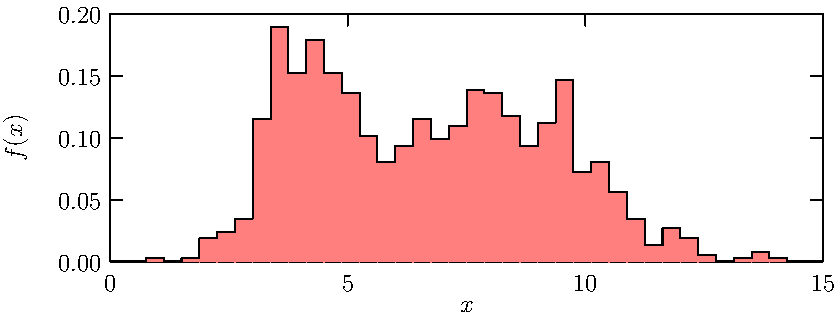
\includegraphics[width=0.6\textwidth]{./figures/mog-0.pdf}
\caption{Example of data measuring the half-lives of two types of particles\label{fig:data}}
\end{figure}
\item Our job is to infer the random variables \(\bm{\Theta}=(\mu_1,
      \mu_2, \sigma_1, \sigma_2, p)\), where \(p=\Prob{Z_i=1}\) is the
probability of the particle being type \(A\)
\item We can do a full Bayesian calculation, but let us just use maximum likelihood
\item The maximum likelihood of the data
\(\mathcal{D}=\{X_i|i=1,2,\ldots,m\}\) is
\begin{align*}
f(\mathcal{D}|\bm{\Theta}) 
&\eq \sum_{\bm{Z}\in\{0,1\}^m}  f(\mathcal{D},\bm{Z}|\bm{\Theta}) \\
&\eq \prod_{i=1}^m \sum_{Z_i\in\{0,1\}} f(X_i, Z_i | \bm{\Theta})
\eq \prod_{i=1}^m  \sum_{Z_i\in\{0,1\}}
f(X_i | Z_i, \bm{\Theta}) \, \Prob{Z_i}
\end{align*}
\explanation
\begin{enumerate}
\item where we marginalise out the latent variables
\(\bm{Z}=(Z_1,Z_2,\ldots Z_n)\)
\item we assume the data is independent
\item we use the identity \(f(X_i, Z_i | \bm{\Theta})= f(X_i | Z_i, \bm{\Theta}) \, \Prob{Z_i}\)
\end{enumerate}
\item It is usually easier working with the log-likelihood
\begin{align*}
\logg{f(\mathcal{D}|\bm{\Theta})} &= \sum_{i=1}^m
\logg{\strut f(X_i|Z_i=1) \, \Prob{Z_i=1} + f(X_i|Z_i=0) \,
\Prob{Z_i=0} }\\
 &=\sum_{i=1}^m
\logg{p\,\normal{X_i}{\mu_A,\sigma_A}+(1-p)\,\normal{X_i}{\mu_B,\sigma_B}}
\end{align*}
\item We could do gradient descent on this, but it is an ugly
expression to work with
\end{itemize}

\subsection{Expectation Maximisation}
\label{sec:org8fc05ac}
\begin{itemize}
\item Rather than maximise the likelihood directly we can iteratively
maximise the expected log-likelihood starting form some initial guess
\(\bm{\Theta}^{(0)}\); we get an improved guess
\begin{equation}
\bm{\Theta}^{(t+1)} = \argmax_{\bm{\Theta}}
\sum_{\bm{Z}\in\{0,1\}^m} \Prob{\bm{Z}\middle|\mathcal{D},\bm{\Theta}^{(t)}}\,
\logg{f(\mathcal{D},\bm{Z} | \bm{\Theta})} \label{eq:em}
\end{equation}
\item This is a general optimisation strategy that is regularly used
when we have latent variables
\item It is known as \textbf{expectation maximisation} or the \textbf{EM-algorithm}
\item This looks very different to maximising the log-likelihood: it
takes some effort to understand why this works
\item To understand this we note
$$f(\mathcal{D},\bm{Z}|\bm{\Theta}) =
      f(\mathcal{D}|\bm{Z},\bm{\Theta}) \, \Prob{\bm{Z}|\bm{\Theta}}  $$
From which we can deduce (taking logs and rearranging)
$$ \logg{f(\mathcal{D}|\bm{Z},\bm{\Theta})} = \logg{f(\mathcal{D},\bm{Z}|\bm{\Theta})} - \logg{\Prob{\bm{Z}|\bm{\Theta}} } $$
\item We now consider the probability distribution
\(\Prob{\bm{Z}\middle|\mathcal{D},\bm{\Theta}^{(t)}}\), that
tells us the probability that \(Z_i=1\) given \(X_i\) and the
parameters \(\bm{\Theta}^{(t)}\) (this is different to the prior
distribution \(\Prob{\bm{Z}|\bm{\Theta}^{t}} = p^{(t)}\))
\item If we not take expectations of
\(\logg{f(\mathcal{D}|\bm{\Theta})}\) give above with respect to
this distribution then
\begin{align*}
  \logg{f(\mathcal{D}|\bm{\Theta})}
   &= \av[\bm{Z}|\bm{\Theta}^{(t)}]{\logg{f(\mathcal{D},\bm{Z}|\bm{\Theta})}}
- \av[\bm{Z}|\bm{\Theta}^{(t)}]{\logg{\Prob{\bm{Z}|\bm{\Theta}} }}
  \\
  &= Q(\bm{\Theta}|\bm{\Theta}^{(t)}) +
  S(\bm{\Theta}|\bm{\Theta}^{(t)})
\end{align*}
\begin{itemize}
\item Note that the left-hand side does not involve the latent
variables so when we take the expectation we get itself
\item The first term on the right-hand side is
$$ Q(\bm{\Theta}|\bm{\Theta}^{(t)}) =
        \av[\bm{Z}|\bm{\Theta}^{(t)}]{\logg{f(\mathcal{D},\bm{Z}|\bm{\Theta})}}
	=  \sum_{\bm{Z}\in\{0,1\}^m} \Prob{\bm{Z}\middle|\mathcal{D},\bm{\Theta}^{(t)}}\,
        \logg{f(\mathcal{D}|\bm{Z}, \bm{\Theta})} $$
\item This is the term we are optimising in equation (\ref{eq:em})
\item The second term is
$$ S(\bm{\Theta}|\bm{\Theta}^{(t)}) = - \av[\bm{Z}|\bm{\Theta}^{(t)}]{\logg{\Prob{\bm{Z}|\bm{\Theta}} }}
	=  - \sum_{\bm{Z}\in\{0,1\}^m} \Prob{\bm{Z}\middle|\mathcal{D},\bm{\Theta}^{(t)}}\,
        \logg{\Prob{\bm{Z}|\bm{\Theta}}} $$
\end{itemize}
\item Using the identity for the log-likelihood we can write the
change in log-likelihood when we update our
parameters 
\begin{align*}
\Delta L &=
\logg{f(\mathcal{D}|\bm{\Theta}^{(t+1)})} -
\logg{f(\mathcal{D}|\bm{\Theta}^{(t)})} \\
&= Q(\bm{\Theta}^{(t+1)}|\bm{\Theta}^{(t)}) -
Q(\bm{\Theta}^{(t)}|\bm{\Theta}^{(t)})
+ S(\bm{\Theta}^{(t+1)}|\bm{\Theta}^{(t)}) -
S(\bm{\Theta}^{(t)}|\bm{\Theta}^{(t)}) \\
&= Q(\bm{\Theta}^{(t+1)}|\bm{\Theta}^{(t)}) -
Q(\bm{\Theta}^{(t)}|\bm{\Theta}^{(t)})
+ \mathrm{KL}\!\left( \Prob{\bm{Z}|\bm{\Theta}^{(t)}} \middle\|
  \Prob{\bm{Z}|\bm{\Theta}^{(t+1)}} \right)
 \end{align*}
\begin{itemize}
\item where
\end{itemize}
\begin{align*}
\mathrm{KL}\!\left( \Prob{\bm{Z}|\bm{\Theta}^{(t)}} \middle\|
\Prob{\bm{Z}|\bm{\Theta}^{(t+1)}} \right) &=
S(\bm{\Theta}^{(t+1)}|\bm{\Theta}^{(t)}) -
S(\bm{\Theta}^{(t)}|\bm{\Theta}^{(t)}) \\
&= -  \sum_{\bm{Z}\in\{0,1\}^m} \Prob{\bm{Z}\middle|\mathcal{D},\bm{\Theta}^{(t)}}\,
\logg{\frac{ \Prob{\bm{Z}|\bm{\Theta}^{(t+1)}} }{ \Prob{\bm{Z}|\bm{\Theta}^{(t)}} }} 
\end{align*}
\begin{itemize}
\item We have shown in a previous lecture that KL-divergences are non-negative
\end{itemize}
\item Now in expectation maximisation we choose
$$ \bm{\Theta}^{(t+1)} = \argmax_{\bm{\Theta}}
      Q(\bm{\Theta}|\bm{\Theta}^{(t)}) $$
which implies \(Q(\bm{\Theta}^{(t+1)}|\bm{\Theta}^{(t)}) \geq
      Q(\bm{\Theta}^{(t)}|\bm{\Theta}^{(t)})\)
\item Thus \(\Delta L\geq 0\), so in each step we increase the log-likelihood
\item This gives us a relative simple procedure for maximising the likelihood
(we can also use this to maximise the \emph{a posteriori} solution);
we choose \(\bm{\Theta}\) to maximise
$$ Q(\bm{\Theta}|\bm{\Theta}^{(t)}) = \sum_{\bm{Z}\in\{0,1\}^m} \Prob{\bm{Z}\middle|\mathcal{D},\bm{\Theta}^{(t)}}\,
      \logg{f(\mathcal{D}|\bm{Z}, \bm{\Theta})} $$
\item Let us return to the problem of working out the half-life statistics of
our two types of particles \(A\) and \(B\)
\item Recall \(f(\mathcal{D},\bm{Z} |\bm{\Theta}) =
      \prod\limits_{i=1}^m  f(X_i|Z_i,\bm{\Theta}) \, \Prob{Z_i}\) where
$$ f(X_i,Z_i|\bm{\Theta}) = p\, Z_i\,\normal{X_i}{\mu_A,\sigma_A^2} +
        (1-p)\,(1-Z_i)\,\normal{X_i}{\mu_B,\sigma_B^2} $$
\item Let 
 \begin{align*}
 p_i^{(t)} &= \Prob{Z_i=1\middle|X_i, \bm{\Theta}^{(t)}} = 
 \frac{p^{(t)}\, \normal{X_i}{\mu_A^{(t)},\sigma_A^{2(t)}} }
{ p^{(t)}\,\normal{X_i}{\mu_A^{(t)},\sigma_A^{2(t)}} + (1-p^{(t)})\, \normal{X_i}{\mu_B^{(t)},\sigma_B^{2(t)}} } \\
 q_i^{(t)} &= \Prob{Z_i=0\middle|X_i, \bm{\Theta}^{(t)}} =
 \frac{(1-p^{(t)})\,\normal{X_i}{\mu_B^{(t)},\sigma_B^{2(t)}}}
{p^{(t)}\, \normal{X_i}{\mu_A^{(t)},\sigma_A^{2(t)}} + (1-p^{(t)})\, \normal{X_i}{\mu_B^{(t)},\sigma_B^{2(t)}} }
 = 1-p_i^{(t)}
 \end{align*}
\item Then
\begin{align*}
Q(\bm{\Theta}|\bm{\Theta}^{(t)}) &= \sum_{i=1}^m \;
p_i^{(t)} \logg{p^{(t)}\,\normal{X_i}{\mu_A,\sigma_A^{2}}}
+ q_i^{(t)}  \logg{(1-p^{(t)})\,\normal{X_i}{\mu_B,\sigma_B^{2}}} \\ 
&= \sum_{i=1}^m \;
p_i^{(t)}\left(\log(p) -
\frac{(X_i-\mu_A)^2}{2\sigma_A^{2}}
  - \frac{1}{2} \logg{2\,\pi\,\sigma_A^{2}} \right) \\
  &\hspace{1cm}
  + q_i^{(t)}\left(\log(1-p) -
  \frac{(X_i-\mu_B)^2}{2\sigma_B^{2}}
  - \frac{1}{2} \logg{2\,\pi\,\sigma_B^{2}} \right) 
  \end{align*}
\item To optimise this we just set the derivatives to 0
\begin{itemize}
\item Optimising with respect to \(p\)
$$ \frac{\partial Q(\bm{\Theta}|\bm{\Theta}^{(t)})}{\partial p}
          = \frac{1}{p} \sum_{i=1}^m \; p_i^{(t)} - \frac{1}{1-p}
          \sum_{i=1}^m \; q_i^{(t)} =0 $$
solving for \(p\)
$$ p^{(t+1)} = \frac{\sum\limits_{i=1}^m 
         p_i^{(t)}}{\sum\limits_{i=1}^m (p_i^{(t)}+q_i^{(t)})} =
         \frac{1}{m} \sum\limits_{i=1}^m  p_i^{(t)}$$
\item Optimising with respect to \(\mu_A\)
$$ \frac{\partial Q(\bm{\Theta}|\bm{\Theta}^{(t)})}{\partial \mu_A} 
	= - \sum\limits_{i=1}^m p_i^{(t)} \frac{X_i-\mu_A}{\sigma_A^{2}} $$
solving for \(\mu_A\) (and performing a similar optimisation
for \(\mu_B\))
$$ \mu_A^{(t+1)} = \frac{ \sum\limits_{i=1}^m
        p_i^{(t)} X_i }{\sum\limits_{i=1}^m p_i^{(t)}} ,\quad\quad
	\mu_B^{(t+1)} = \frac{ \sum\limits_{i=1}^m
        q_i^{(t)} X_i }{\sum\limits_{i=1}^m q_i^{(t)}} $$
\item Putting in the optimal value for \(\mu^{(t)}_A\) and optimising with respect to \(\sigma_A^2\)
 $$ \frac{\partial Q(\bm{\Theta}|\bm{\Theta}^{(t)})}{\partial \sigma^2_A}
	 = \frac{1}{2\,\sigma^4_A}\sum_{i=1}^m p_i^{(t)}
         (X_i-\mu^{(t)}_A)^2- \frac{1}{\sigma_A^{2}}\sum_{i=1}^m p_i^{(t)}$$
Solving for \(\sigma^2_A\) (and performing a similar optimisation
for \(\sigma^2_B\))
$$ \sigma_A^2 = \frac{ \sum\limits_{i=1}^m
        p_i^{(t)} (X_i-\mu^{(t)}_A)^2 }{\sum\limits_{i=1}^m p_i^{(t)}}
        ,\quad\quad
	 \sigma_B^2 = \frac{ \sum\limits_{i=1}^m
        q_i^{(t)} (X_i-\mu^{(t)}_B)^2 }{\sum\limits_{i=1}^m q_i^{(t)}}$$
\end{itemize}
\item These are very natural update equations
\begin{itemize}
\item we make an estimate, \(p_i^{(t)\) of the probability that observation \(X_i\)
is a particle of type \(A\) or \(B\) base on our current parameters
\item we then update all our parameters based on these estimates
\end{itemize}
\item We are guaranteed that our EM-algorithm never decreases the
likelihood (although it could reach a local rather than global optimum)
\item For the data set we showed earlier (which was a random sample
of size 1000 generated using \(p=0.3\), \(\mu_A=4\),
\(\sigma_A=0.8\), \(\mu_B=8\) and \(\sigma_B=2\)) we get the results
shown in Figure \ref{fig:mog}
\begin{figure}[htbp]
\centering
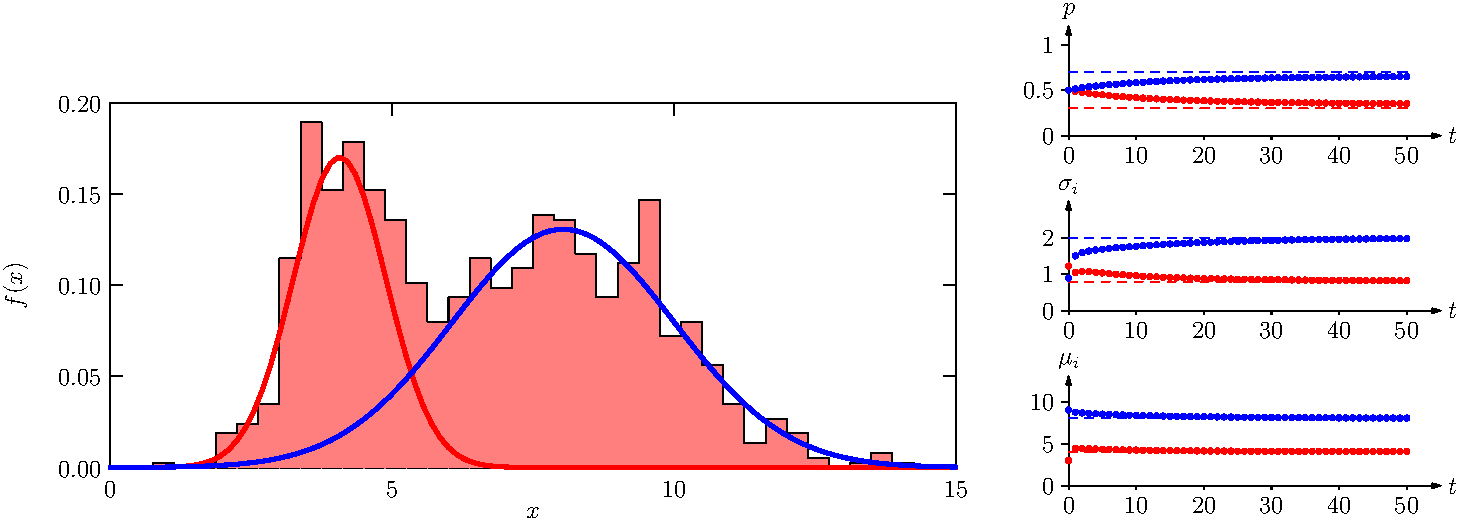
\includegraphics[width=0.95\textwidth]{./figures/mog-1.pdf}
\caption{Example of EM algorithm to compute the statistics for the half-lives of our two particles \label{fig:mog}}
\end{figure}
\item The EM algorithm often leads to very natural update equations,
but its convergence is often rather slow
\end{itemize}

\section{Exercises}
\label{sec:org7fb6db1}

\subsection{Mysterious Disease}
\label{sec:orge2d3c1c}
\begin{itemize}
\item We assume that we are tracking some disease
\item Let \(Z(t)\) be the number of people that catch the
disease on day \(t\), but this is unknown (a latent variable)
\item We assume the rate of growth of the disease is
$$ \Prob{Z(t+1)} = \mathrm{Poi}\!\left(Z(t+1)\middle|
     \frac{r_0}{3}\, (Z(t)+Z(t-1)+Z(t-2)) \right) $$
\begin{itemize}
\item We are assuming that someone is virulent for the first three
days after catching the disease
\item We assume \(Z(1)=1\) and \(Z(0)=Z(-1)=0\)
\item In expectation everyone with the disease will infect \(r_0\) new people
\end{itemize}
\item We observe \(X(t)\) which is some proportion of new patients such that
$$ \Prob{X(t) = k} = \mathrm{Binom}(k|Z(t), p) = \binom{Z(t)}{k}
     p^k\,(1-p)^{Z(t)-k} $$
\begin{itemize}
\item We assume that each patient will be tested with a probability \(p\)
\item We are given a time series \((X(1), X(2), \ldots, X(T))\)
\end{itemize}
\item Build a probabilistic model to estimate \(p\) and \(k_0\)
\item See answers
\end{itemize}

\subsection{Experiments}
\label{sec:org6d48696}

\subsection{Mysterious Disease}
\label{sec:orgf8dca74}
\begin{itemize}
\item Build a simulator of your models (assume you know \(p\) and \(r_0\))
\item Choose any language you are comfortable with
\item If you are feeling very adventurous you could try to solve your
model to predict \(p\) and \(r_0\), but be warned this is hard (you
probably need to use MCMC, but you could try an EM algorithm)
\end{itemize}

\begin{minted}[]{octave}
r0 = 2
r = r0/3
p = 0.2
T = 20
Z(1) = 1;
Z(2) = poissrnd(r*Z(1));
Z(3) = poissrnd(r*(Z(1)+Z(2)));
for t = 4:T
   Z(t) = poissrnd(r*(Z(t-1)+Z(t-2)+Z(t-3)));
endfor

for t= 1:T
  X(t) = binornd(Z(t),p);
endfor
\end{minted}

\section{Answers}
\label{sec:org74cb4cf}

\subsection{Mysterious Disease}
\label{sec:orgb02f1d5}
\begin{itemize}
\item We want to compute \(f(p,k_0|\mathcal{D})\) where
\(\mathcal{D}=(X(1), X(2), \ldots, X(T))\)
\item We have a likelihood of 
$$ \Prob{X(t)\middle|Z(t),p} = \mathrm{Binom}(X(t)|Z(t), p) $$
where
$$ \Prob{Z(t+1)|r_0,Z(t),Z(t-1),Z(t-2)} = \mathrm{Poi}\!\left(Z(t+1)\middle|
     \frac{r_0}{3}\, (Z(t)+Z(t-1)+Z(t-2)) \right) $$
\item To perform a Bayesian calculation we would have to put priors,
\(f(p)\) and \(f(r_0)\), on \(p\) and \(r_0\)
\begin{itemize}
\item A reasonable prior to use for \(p\) is \(f(p) =
       \mathrm{Beta}(p|a,b)\)---you could use \(a=b=0\) as an uninformative
priors, but you might have some prior knowledge, e.g. \(a=b=2\) say
which says \(f(p)=6\,p\,(1-p)\)
\item A reasonable prior for \(r_0\) would be
\(\mathrm{Gamma}(r_0|a,b)\)---you could use \(a=b=0\) as an
uninformative prior but again you might have some prior belief, e.g. \(a=2\), \(b=1\)
\end{itemize}
\item Bayes rule tells us
$$ f(p,r,\bm{Z}|\bm{X}) = \frac{\Prob{X(t)\middle|Z(t),p}\, \prod\limits_{t=1}^T
     \Prob{Z(t)|Z(t-1),Z(t-2),Z(t-3),r_0} \,
     f(r_0)\,f(p)}{\Prob{\bm{X}}} $$
\item To get estimates of \(p\) and \(r_0\) we have to marginalise out \(\bm{Z}\)
\item Now the problem is this is rather horrible to compute (your
priors are not conjugate priors in this problem and the posterior
is very complicated)
\item Probably the best way to do this is to use Markov Chain Monte
Carlo (MCMC), but you will have to wait before I get there
\end{itemize}
\end{document}
